\begin{figure}[h]
  \centering
  \begin{tabular}{ c p{0.15cm} c p{0.15cm} c }
    %\centering
    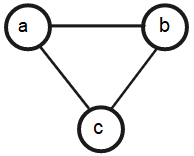
\includegraphics[width=2.3cm]{./img/trianguloabc.png} && 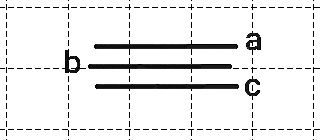
\includegraphics[width=3.5cm]{./img/b0epgTransparenciaGrade2.png} & &
    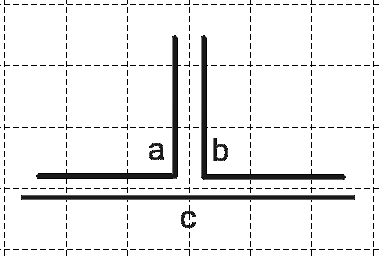
\includegraphics[width=3.5cm]{./img/b1EpgTransparenteGrade2.png}
    \\
    \footnotesize %\centering 
    (a) O grafo $C_3$ && \footnotesize(b) Representação $B_0$-EPG de $C_3$ && \footnotesize (c) Representação $B_1$-EPG de $C_3$\\

  \end{tabular}

 \caption{O grafo $ C_3 $ com duas representações, uma sem dobra e outra com uma dobra} \label{fig:trianguloepgRepresentacao}
\end{figure}